%%%%%%%%%%%%%%%%%%%%%%%%%%%%%%%%%%%%%%%%%%%%%%%%%%%%%%%%%%%%%%%%%%%%%%%%%%%%%%%
%2345678901234567890123456789012345678901234567890123456789012345678901234567890
%        1         2         3         4         5         6         7         8

\documentclass[letterpaper, 12 pt, conference]{ieeeconf}  % Comment this line out
                                                          % if you need a4paper
%\documentclass[a4paper, 10pt, conference]{ieeeconf}      % Use this line for a4
                                                          % paper

\IEEEoverridecommandlockouts                              % This command is only
                                                          % needed if you want to
                                                          % use the \thanks command
\overrideIEEEmargins
% See the \addtolength command later in the file to balance the column lengths
% on the last page of the document

\usepackage[utf8]{inputenc}
\usepackage[T1]{fontenc}
\usepackage{graphicx}
\usepackage{float}


% The following packages can be found on http:\\www.ctan.org
%\usepackage{graphics} % for pdf, bitmapped graphics files
%\usepackage{epsfig} % for postscript graphics files
%\usepackage{mathptmx} % assumes new font selection scheme installed
%\usepackage{mathptmx} % assumes new font selection scheme installed
%\usepackage{amsmath} % assumes amsmath package installed
%\usepackage{amssymb}  % assumes amsmath package installed

\title{\LARGE \bf
Analysis of Forksheet Dielectric Wall Materials
}

\author{ \parbox{3 in}{\centering Christopher Calloway \\
        % \thanks{}\\ 
        Electrical Engineering\\
        Stanford University\\
        {\tt\small cmc2374@stanford.edu}}
        \hspace*{ 0.5 in}
        \parbox{3 in}{ \centering Vanessa Barnard\\
        % \thanks{}\\
        Electrical Engineering \\
        Stanford University\\
        {\tt\small @stanford.edu}}
          \hspace*{ 0.5 in}
        \parbox{3 in}{ \centering adsfasdfa\\
        % \thanks{}\\
        Electrical Engineering \\
        Stanford University\\
        {\tt\small adsf@stanford.edu}}
}

% \author{ Chris Calloway$^{1}$, Yiwen Jiang$^{2}$, Louise Zhuang$^{3}$% <-this % stops a space
% \thanks{* Supervised by Mert Pilanci, Yifei Wang}% <-this % stops a space
% \thanks{$^{1}$ Chris Calloway
%         {\tt\small cmc2374 at stanford dot edu}}%
        
% \thanks{$^{2}$ Yiwen Jiang
%         {\tt\small  at stanford dot edu}}%

% \thanks{$^{3}$ Louise Zhuang
%         {\tt\small  at stanford dot edu}}%
        
    
% }


\begin{document}



\maketitle
\thispagestyle{empty}
\pagestyle{empty}


%%%%%%%%%%%%%%%%%%%%%%%%%%%%%%%%%%%%%%%%%%%%%%%%%%%%%%%%%%%%%%%%%%%%%%%%%%%%%%%%
\begin{abstract}

In this project, we will analyze the choice of material for the dielectric wall in forksheet (FSH) devices. FSH are an alternate device structure to FinFET and GAA device which due to its dielectric wall allows for tight PMOS/NMOS separation and thus more scaling. The dielectric constant of the wall, which is determined by the material, has an impact on both the subthreshold slope and coupling effects through the dielectric wall. In particular, a high k dielectric degrades subthreshold slope but improves coupling effects within the wall, whereas the opposite is true for a low k dielectric. We seek to find the optimal wall material to optimize a forksheet device for both good subthreshold slope and coupling behavior. 


\end{abstract}


%%%%%%%%%%%%%%%%%%%%%%%%%%%%%%%%%%%%%%%%%%%%%%%%%%%%%%%%%%%%%%%%%%%%%%%%%%%%%%%%
\section{INTRODUCTION}

\subsection{Overview}






\subsection{Related Work}




\section{Process and Simulation}

To analyze the choice of material within the a FSH structure, we first created a generic FSH structure in Sentaurus. We then measured Id vs Vgs characteristics for several versions of this generic device with the dielectric wall material swapped out. We also measured the capacitance between the walls of the dielectric and the current flow to get a measurement of the coupling. Finally, using these results we arrived 


The generic FSH CAD structure can be seen in Figure 1. This 3D view contains both the doping information as well as the device dimensions. The dielectric wall (shown in yellow) is set to be SiN in this default case, but will be changed for all other simulations while keeping the width, 17nm, constant. Figure 2 shows the interior of the FSH as viewed as a slice into the gate region of the device. Figure 2 outlines the specifics of the gate stack dimensions and materials used. This structure was based on the findings of \cite{c1}, which showed the state of the art structure for FSH devices. The choice of materials was determined from \cite{c2}. Specifically, this textbook chapter on setting work functions for Hi-K gate metals recommends to use a High K material of HFO2, and a cap of TiN. \cite{c2} also recommends to use Lanthanum (La) and Aluminum (Al) for NMOS and PMOS, respectively. However, Sentaurus does not currently of a Lanthanum material for simulation. However, \cite{c3} suggests that Tantalum (Ta) is also a reasonable work function metal for NMOS, and Sentaurus has a Ta simulation capability. Therefore, we use Ta for our NMOS work function metal. 

The following materials were used for gate dielectric materials (in order of their dielectric constant)

\begin{enumerate}
    \item Air Gap, k=1
    \item Low Porosity Si02, k=2
    \item Si02, k=3.9
    \item Ge02, k=4.5
    \item Si3N4, k=7.5
    \item Ga2O3, k=15
    \item HfO2, k = 25
    \item TiO2, k = 80
\end{enumerate}

To extract the relevant information for the Id vs Vgs curve, we applied a bias of  to

To extract the relevant information for the coupling effects.

An analysis of the results for these 8 materials can be found Section 3.
 



\section{Fabrication Considerations}



\section{Results}

% \newline \,\,



\section{Conclusion and Future Work}



\section*{ACKNOWLEDGMENT}

The authors would like to thank Professor H.-S. Phillip Wong for their guidance on this project.



\begin{thebibliography}{99}


\bibitem{c1} P. Weckx et al., "Novel forksheet device architecture as ultimate logic scaling device towards 2nm," 2019 IEEE International Electron Devices Meeting (IEDM), 2019, pp. 36.5.1-36.5.4, doi: 10.1109/IEDM19573.2019.8993635.


\bibitem{c2} E. Erben, K. Hempel, and D. Triyoso, "Work Function Setting in High-k Metal Gate Devices", in Complementary Metal Oxide Semiconductor. London, United Kingdom: IntechOpen, 2018 [Online]. Available: https://www.intechopen.com/chapters/61888 doi: 10.5772/intechopen.78335

\bibitem{c3} G. Thareja, H. C. Wen, R. Harris, P. Majhi, B. H. Lee and J. C. Lee, "NMOS Compatible Work Function of TaN Metal Gate With Gadolinium Oxide Buffer Layer on Hf-Based Dielectrics," in IEEE Electron Device Letters, vol. 27, no. 10, pp. 802-804, Oct. 2006, doi: 10.1109/LED.2006.882521.


\end{thebibliography}

\newpage
\section{Appendix}

\begin{figure}[H]
    \centering
    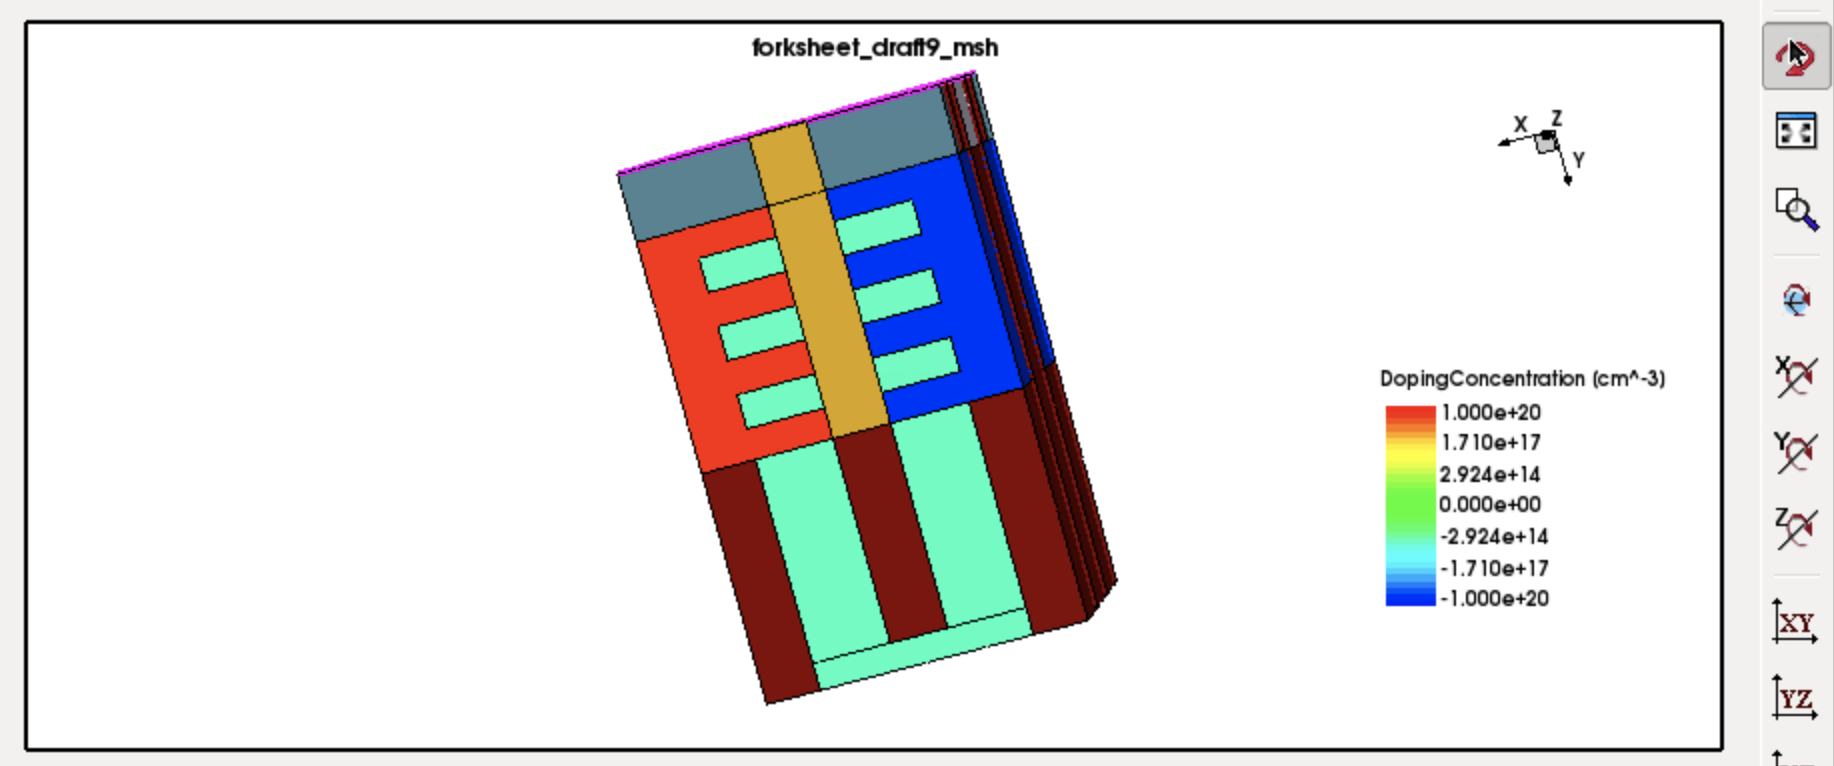
\includegraphics[width=.9\linewidth]{Screen Shot 2022-02-26 at 3.13.29 PM.png}
    \caption{Plot showing full 3D CAD structure of the FSH. Includes doping and gate contact information as well}
    \label{fig:knngraph1}
\end{figure}

\begin{figure}[H]
    \centering
    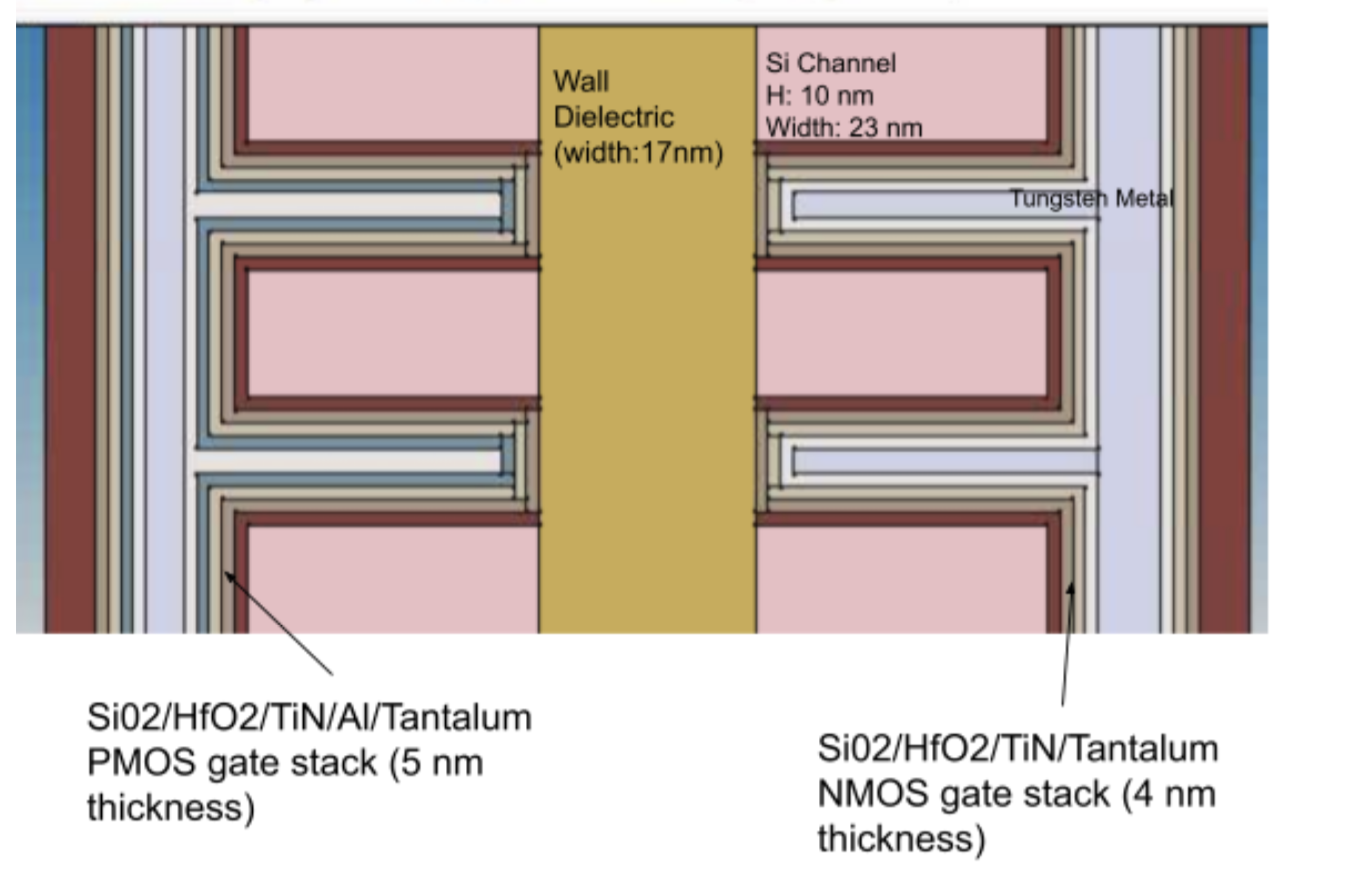
\includegraphics[width=.9\linewidth]{Screen Shot 2022-02-26 at 9.27.22 PM.png}
    \caption{Plot showing the specific gatestack for our CAD model}
    \label{fig:knngraph1}
\end{figure}

\begin{figure}[H]
    \centering
    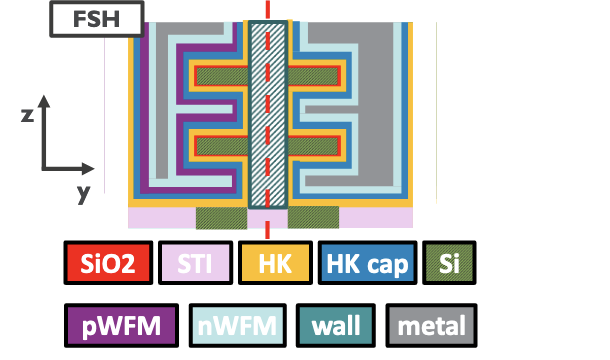
\includegraphics[width=.9\linewidth]{Screen Shot 2022-02-26 at 10.04.03 PM.png}
    \caption{State of the Art Interior of FSH as described by \cite{c1} }
    \label{fig:knngraph1}
\end{figure}




\end{document}
